\documentclass{article}
\usepackage{setspace}
\usepackage{amsmath}
\usepackage{graphicx} 
\usepackage{float} 
\usepackage{fancyhdr}                                
\usepackage{lastpage}                                           
\usepackage{layout}   
\usepackage{subfigure} 
\pagestyle{fancy}  
\lhead{ZHANG HUAKANG}
\chead{Assignment 3} 
\rhead{DB92760} 
\renewcommand{\baselinestretch}{1.05}
\title{Assignment 3 of MATH 2005}
\author{ZHANG Huakang/DB92760}

\begin{document}
    \maketitle

    \section{}
    \subsection{}
        \paragraph{By the Proposition 3.1.1,}
        \paragraph{$$\sum _{x=1} ^5 f(x)=1.$$}
        \paragraph{Therefore, $k=\frac{1}{15}$.}

    \subsection{}
        \paragraph{$$\sum _{x=0} ^5 f(x)=1.$$}
        \paragraph{Thus, $k=\frac{1}{32}$.}

    \subsection{}
        \paragraph{$$\sum _{x=1} ^n f(x)=\sum _{x=1} ^n kx^2=k\sum _{x=1}^n x^2=k\frac{n(x+1)(2n+1)}{6}=1 .$$}
        \paragraph{Thus, $k=\frac{6}{n(n+1)(2n+1)}$.}

    \subsection{}
        \paragraph{$$\sum _{x=1} ^\infty f(x)=\sum _{x=1} ^\infty k (\frac{1}{4})^x=k\sum _{x=1} ^\infty (\frac{1}{4})^x=k \lim _{x\rightarrow \infty} \frac{\frac{1}{4}\times(1-(\frac{1}{4})^x)}{1-\frac{1}{4}}=k\times 3 =1$$}
        \paragraph{Thus, $k=\frac{1}{3}$.}

    \section{}
    \paragraph{
        $f(1)=\frac{1}{15}$,   \\    
        $f(2)=\frac{2}{15}$ ,   \\
        $f(3)=\frac{1}{5}$  ,  \\
        $f(4)=\frac{4}{15}$ ,  \\
        $f(5)=\frac{1}{3}$  .\\
        And we can find that $\sum _{x=1} ^ 5 f(x)=1$
    }

    \paragraph{Therefore,\\
        $F(x)=0$ when $x< 1$.\\
        $F(x)=f(1)=\frac{1}{15}$ when $1\leq x< 2$.\\
        $F(x)=f(1) +f(2)=\frac{1}{5}$ when $2\leq x< 3$.\\
        $F(x)=f(1)+f(2)+f(3)=\frac{2}{5}$ when $3\leq x< 4$.\\
        $F(x)=f(1)+f(2)+f(3)+f(4)=\frac{2}{3}$ when $4\leq x< 5$.\\
        $F(x)=f(1)+f(2)+f(3)+f(4)+f(5)=1$ when $x\geq 5$.
    }

    \section{}
        \subsection{}
            \paragraph{
                By the definition,
                $$P(2<X\leq 6)=P(x\leq 6)-P(x\leq 2)=F(6)-F(2)=\frac{1}{2}$$
                $$P(X=4)=\frac{1}{6}$$
            }
        \subsection{}
            \paragraph{
                By the Proposition 3.1.3, we know that if $X={x_n \in R:n=1,2,...}$ with $x_1<x_2<...<x_n<...$, then $f(x_k)=F(x_k)-F(x_{k-1})$.
            }
            \paragraph{
                Therefore,we can get 
                $$f(1)=\frac{1}{3}.$$
                Similarly, $f(4)=\frac{1}{6},f(6)=\frac{1}{3},f(10)=\frac{1}{6}$.  When $x\neq 1$ and $x\neq 4$ and $x\neq 6$ and $x\neq 10$,
                $f(x)=0$ .
            }
    \section{}
        \subsection{}
            \paragraph{
                By the Proposition 3.2.2,
                $$\int _{-\infty} ^\infty f(x)=\int _{-\infty} ^0 0 dx +\int _ 0 ^4 \frac{c}{\sqrt{x}} dx + \int _4 ^\infty 0 dx=0+ 2c\sqrt{x}| _0 ^4 +0=4c=1$$
                Hence, we get $c=\frac{1}{4}$
            }
        \subsection{}
            \paragraph{
                By the definition and Proposition 3.2.1,
                $$P(X<\frac{1}{4})=P(X\leq\frac{1}{4})=\int _{-\infty}  ^\frac{1}{4}f(x)dx=\frac{1}{4}$$
                $$P(X>1)=1-P(X\leq 1)=1-\int _{-\infty}  ^1f(x)dx=\frac{1}{2}$$
            }
        \subsection{}
            \paragraph{
                When $x\leq0$, 
                $$F(x)=\int _{-\infty} ^x 0 dx= 0$$
                When $0<x<4$,
                $$F(x)=F(0)+\int _0 ^x \frac{1}{4\sqrt{x}} dx =\frac{\sqrt{x}}{2}$$
                When $x \geq 4$
                $$F(x)=F(4)+\int _4 ^\infty 0 dx =1$$
            }
    \section{}
        \subsection{}
            \paragraph{
                By the Proposition 3.2.1,
                $$\int _{-\infty} ^\infty f(z) dz=\int _0 ^\infty kze^{-z^2} =1$$
                Thus, $k=2$ and $f(x)=2ze^{-z^2}$ when $z>0$
            }
            \begin{figure}[H] 
                \centering 
                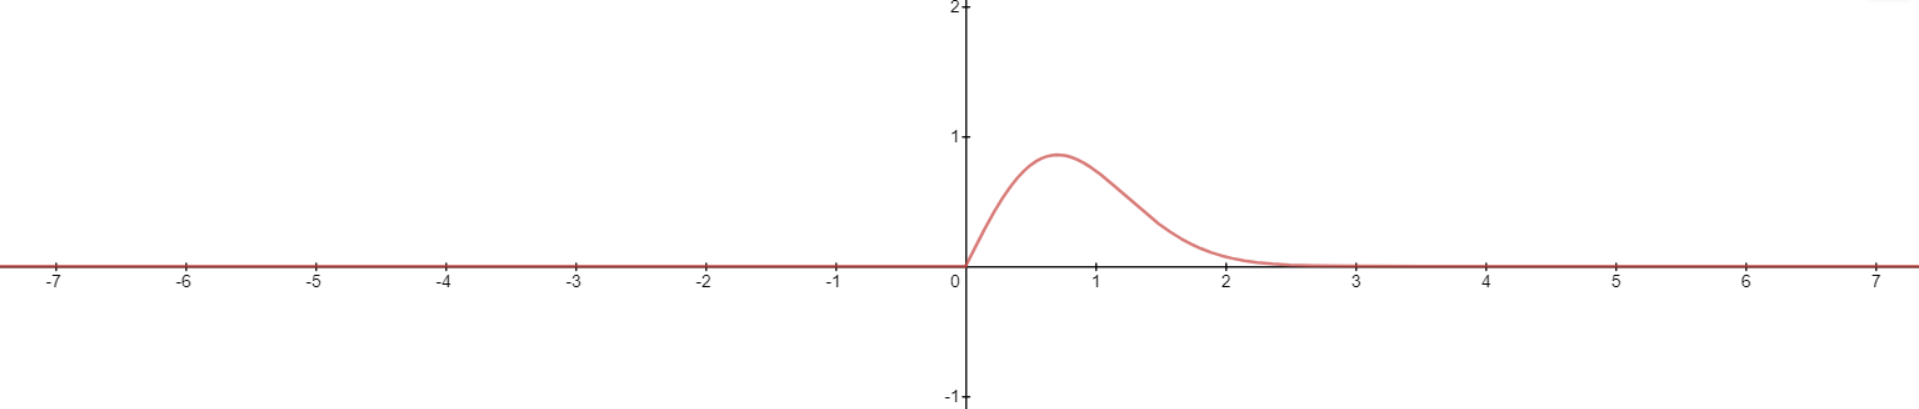
\includegraphics[width=0.9\textwidth]{Assignment3-1.png} 
                \caption{Density Function} 
            \end{figure}
        \subsection{}
            \paragraph{
                By the definition,\\
                $F(z)=P(Z<z)=\int _{-\infty} ^z 0 dz =0$ when $z\leq0$.\\
                $F(z)=F(0)+\int _0 ^z 2ze^{-z^2} dz = 1- e^{-z^2}$ when $z>0$
            }
            \begin{figure}[H] 
                \centering 
                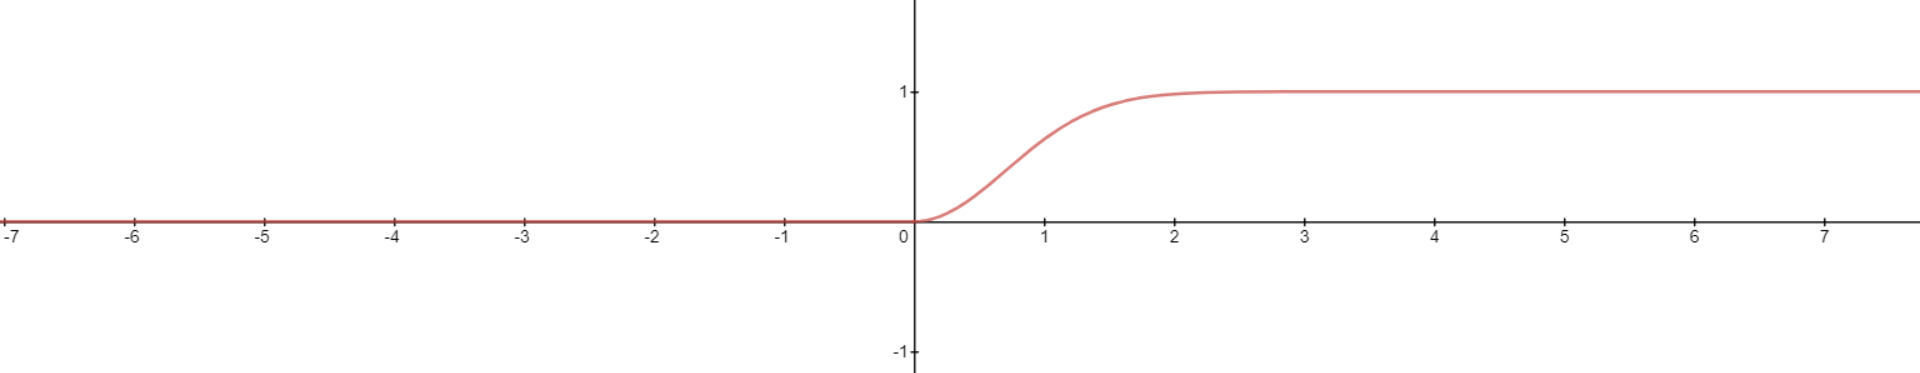
\includegraphics[width=0.9\textwidth]{Assignment3-2.png} 
                \caption{Distribution Function} 
            \end{figure}
    \section{}
        \subsection{}
            \paragraph{
                $$P(X\leq 2)=F(2)=1-3e^{-2}$$
                $$P(1<X<3)=P(1\leq X \leq 3 )=F(3)-F(1)=2e^{-1}-4e^{-3}$$
                $$P(X>4)=1-P(X\leq 4)=5e^{-4}$$
            }
        \subsection{}
            \paragraph{
                By the Proposition 3.2.1,
                $f(x)=\frac{d}{dx}F(x)$.
                We can get that
                $$f(x)=\frac{d}{dx} 0 =0$$
                when $x\leq0$.
                $$f(x)=\frac{d}{dx}(1-(1+x)e^{-x})=xe^{-x}$$
                when $x>0$.
            }
    \section{}
        \subsection{}
            \paragraph{
                $$P(x\leq 6)=\int _{-\infty} ^6 f(x)dx=0+\int _0 ^6 \frac{1}{9}xe^{-\frac{1}{3}x} dx=1-3e^{-2}$$
            }
        \subsection{}
            \paragraph{
                $$P(x\geq 9)=1-P(x<9)=1-P(x\leq 9)=1-\int _{-\infty} ^9 f(x)dx=4e^{-3}$$
            }
    \section{}
        \subsection{}
            \paragraph{
                $$P(X> 10)=1-P(X\leq 10)=1-F(10)=0.25$$
            }   
        \subsection{}
            \paragraph{
                $$P(X < 8)=P(X \leq 8)=F(8)=\frac{39}{64}$$
            }
        \subsection{}
            \paragraph{
                $$P(12\leq X \leq 15)=F(15)-F(12)=\frac{1}{16}$$
            }
    \section{}
        \subsection{}
        \begin{tabular}{|c|c|c|c|c|}
            \hline        & $x=0$ & $x=1$ & $x=2$ & $x=3$ \\
            \hline  $y=0$ & $0$ & $\frac{1}{30}$ & $\frac{1}{15}$ & $\frac{1}{10}$ \\
            \hline  $y=1$ & $\frac{1}{30}$ & $\frac{1}{15}$ & $\frac{1}{10}$ & $\frac{2}{15}$ \\
            \hline  $y=2$ & $\frac{1}{15}$ & $\frac{1}{10}$ & $\frac{2}{15}$ & $\frac{1}{6}$ \\
            \hline
        \end{tabular}
        \subsection{}
            \paragraph{
                Let $g(x)$ and $h(y)$ be the marginal probability distributions of $X$ and $Y$ respectively.
                Thus,\\
            }
            \begin{tabular}{|c|c|c|c|c|c|}
                \hline        & $x=0$ & $x=1$ & $x=2$ & $x=3$ & $h(y)$\\
                \hline  $y=0$ & $0$ & $\frac{1}{30}$ & $\frac{1}{15}$ & $\frac{1}{10}$ &$\frac{1}{5}$\\
                \hline  $y=1$ & $\frac{1}{30}$ & $\frac{1}{15}$ & $\frac{1}{10}$ & $\frac{2}{15}$ & $\frac{1}{3}$ \\
                \hline  $y=2$ & $\frac{1}{15}$ & $\frac{1}{10}$ & $\frac{2}{15}$ & $\frac{1}{6}$ &$\frac{7}{15}$\\
                \hline  $g(x)$&$\frac{1}{10}$ & $\frac{1}{5}$ & $\frac{3}{10}$ &$\frac{2}{5}$ & \\
                \hline
            \end{tabular}
    \section{}
            \begin{equation}
                \begin{split}
                    P(X+Y<\frac{1}{2})
                    &=\int _{-\infty} ^{\frac{1}{2}} \int _{-\infty} ^{\frac{1}{2}-y} f(x,y) dx dy\\
                    &=\int _0 ^{\frac{1}{2}} \int _0 ^{\frac{1}{2}-y} f(x,y) dx dy\\
                    &=\int _0 ^\frac{1}{2} 12x^2y|_{x=0} ^{\frac{1}{2}-y} dy\\
                    &=\int_{0} ^\frac{1}{2} 12(\frac{1}{4}y-y^2 +y^3)dy\\
                    &=12(\frac{1}{8}y^2-\frac{1}{3}y^3+\frac{1}{4}y^4)|_{y=0} ^ \frac{1}{2}\\
                    &=\frac{1}{16}
                \end{split}
            \end{equation}
    \section{}
        \paragraph{
            By the Proposition 3.3.3,
            $$f(x,y)=\frac{\partial}{\partial x \partial y}F(x,y)=0$$
            when $x\leq 0 $ or $y\leq 0$.
            $$f(x,y)=\frac{\partial}{\partial x \partial y}F(x,y)=2xye^{-x^2-y^2}$$
            when $x>0$ and $y>0$.
        }
        \paragraph{
            Let $g(x)$ and $h(y)$ be the marginal densities of $X$ and $Y$ respectively.
            Thus, 
            $$g(x)=\int _{-\infty} ^\infty f(x,y) dy= \int _0 ^\infty f(x,y) dy=2xe^{-x^2-y^2}(1-2y),$$
            $$h(y)=\int _{-\infty} ^\infty f(x,y) dx= \int _0 ^\infty f(x,y) dx =2ye^{-x^2-y^2}(1-2x)$$
        }
        \paragraph{
            \begin{equation}
                \begin{split}
                    g(x)h(y)
                    &=2xe^{-x^2-y^2}(1-2y)\times 2ye^{-x^2-y^2}(1-2x)\\
                    &=4xye^{-2x^2-2y^2}(1-2x)(1-2y)\\
                    & \neq f(x,y)
                \end{split}
            \end{equation}
            Therefore, $X$ and $Y$ are not independent.
        }
    \section{}
        \subsection{}
            \paragraph{
                \begin{equation}
                    \begin{split}
                        P(X\leq 0.3, S >2)
                        &=1-P(X\leq 0.3 , S \leq 2)\\
                        &=1-\int _{-\infty} ^{0.3} \int _{-infty} ^2 f(x,s) ds dx\\
                        &=1-\int _0 ^{0.3} \int _0 ^2 f(x,s) ds dx\\
                        &\approx 0.62798
                    \end{split}
                \end{equation}
            }
        \subsection{}   
            \paragraph{
                Let $g(x)$ be the marginal distributions of $X$. By the definition,
                $$g(x)=0.$$
                when $x\leq 0.20$ or $x\geq 0.40$,
                $$g(x)=\int _{-\infty} ^{\infty} f(x,s) ds=5$$
                when $0.20<x<0.40$\\
                By the definition, when $s\leq 0$,
                $$f(s|x)=\frac{f(x,y)}{g(x)}=0.$$
                when $s>0$,
                $$f(s|x)=xe^{-xs}.$$
            }      
        \subsection{}
            \paragraph{
                \begin{equation}
                    \begin{split}
                        P(S\leq 3|x=25)
                        &=\int_{-\infty} ^3 f(s|25) ds\\
                        &=\int_0 ^3 25e^{-25s} ds\\
                        &=1-e^{-75}\\
                        &\approx 1
                    \end{split}
                \end{equation}
            }
    \section{}
        \subsection{}
            \paragraph{
                Let $f(X,W)$ be the joint probability distribution of $Z$ and $W$.
                $$f(0,0)=\frac{48}{52}\times \frac{47}{51}=\frac{188}{221}$$
                $$f(1,1)=\frac{4}{52}\times\frac{48}{51}=\frac{16}{221}$$
                $$f(0,1)=\frac{48}{52}\times\frac{4}{51}=\frac{16}{221}$$
                $$f(1,2)=\frac{4}{52}\times\frac{3}{51}=\frac{1}{221}$$
            }
        \subsection{}
            \paragraph{
                Let $g(z)$ be the marginal distribution of $Z$,
                $$g(0)=\frac{12}{13}$$
                $$g(1)=\frac{1}{13}$$
            }
        \subsection{}
            \paragraph{
                By the definition,
                $$f(w|z)=\frac{f(z,w)}{g(z)}$$
                Thus, $f(w=1|z=1)=\frac{f(1,1)}{g(1)}=\frac{16}{17}$ and $f(w=2|z=1)=\frac{f(2,1)}{g(1)}=\frac{1}{17}$
            }
    \section{}
        \subsection{}
            \paragraph{
                Let $g(x)$ and $h(x)$ be the marginal densities of $X$ and $Y$, respectively.
                $$g(x)=\int _{-\infty} ^\infty f(x,y) dy=\int _0 ^{1-x} f(x,y)dy=4(1-x)^3$$
                and
                $$h(y)=\int _{-\infty} ^\infty f(x,y) dx = \int _0 ^{1-y} f(x,y) dx=12(1-y)^2y$$
            }
        \subsection{}
            \paragraph{
                If $x>0$, $y>0$ and $x+y<1$
                \begin{equation}
                    \begin{split}
                        g(x)h(x)-f(x,y)
                        &= 48(1-x)^3(1-y)^2y-24y(1-x-y)\\
                        &\neq 0
                    \end{split}
                \end{equation}
                Therefore, $X$ and $Y$ are not independent
            }
    \section{}
        \subsection{}
            \paragraph{
                By the definition of Independence, if $0<x<2$ and $0<y<3$,
                $$f(x,y)=g(x)h(y)=\frac{1}{6}$$
                If $x\leq 0$ or $x\geq 2$ or $y\leq 0$ or $y\geq 3$
                $$f(x,y)=0$$
            }
        \subsection{}
            \paragraph{
                \begin{equation}
                    \begin{split}
                        P(X^2+Y^2>1)&=\int _{-\infty} ^\infty \int _{-\infty} ^\infty f(x,y)dy dx\\
                        &=\int _0 ^1 \int _{\sqrt{1-x^2}} ^3 \frac{1}{6} dy dx+\int _1 ^2 \int _0 ^3 \frac{1}{6} dy dx\\
                        &=\int _0 ^1 \frac{1}{6}y| _{\sqrt{1-x^2}} ^3 dx+\int _1 ^2 \frac{1}{6}y| _{0} ^3 dx\\
                        &=\int _0 ^1 \frac{1}{2}-\frac{\sqrt{1-x^2}}{6} dx +\frac{1}{2}\\
                        &\approx 0.8691
                    \end{split}
                \end{equation}
            }
\end{document}

